
\documentclass[11pt]{article}\usepackage[]{graphicx}\usepackage[]{xcolor}
% maxwidth is the original width if it is less than linewidth
% otherwise use linewidth (to make sure the graphics do not exceed the margin)
\makeatletter
\def\maxwidth{ %
  \ifdim\Gin@nat@width>\linewidth
    \linewidth
  \else
    \Gin@nat@width
  \fi
}
\makeatother

\definecolor{fgcolor}{rgb}{0.345, 0.345, 0.345}
\newcommand{\hlnum}[1]{\textcolor[rgb]{0.686,0.059,0.569}{#1}}%
\newcommand{\hlstr}[1]{\textcolor[rgb]{0.192,0.494,0.8}{#1}}%
\newcommand{\hlcom}[1]{\textcolor[rgb]{0.678,0.584,0.686}{\textit{#1}}}%
\newcommand{\hlopt}[1]{\textcolor[rgb]{0,0,0}{#1}}%
\newcommand{\hlstd}[1]{\textcolor[rgb]{0.345,0.345,0.345}{#1}}%
\newcommand{\hlkwa}[1]{\textcolor[rgb]{0.161,0.373,0.58}{\textbf{#1}}}%
\newcommand{\hlkwb}[1]{\textcolor[rgb]{0.69,0.353,0.396}{#1}}%
\newcommand{\hlkwc}[1]{\textcolor[rgb]{0.333,0.667,0.333}{#1}}%
\newcommand{\hlkwd}[1]{\textcolor[rgb]{0.737,0.353,0.396}{\textbf{#1}}}%
\let\hlipl\hlkwb

\usepackage{framed}
\makeatletter
\newenvironment{kframe}{%
 \def\at@end@of@kframe{}%
 \ifinner\ifhmode%
  \def\at@end@of@kframe{\end{minipage}}%
  \begin{minipage}{\columnwidth}%
 \fi\fi%
 \def\FrameCommand##1{\hskip\@totalleftmargin \hskip-\fboxsep
 \colorbox{shadecolor}{##1}\hskip-\fboxsep
     % There is no \\@totalrightmargin, so:
     \hskip-\linewidth \hskip-\@totalleftmargin \hskip\columnwidth}%
 \MakeFramed {\advance\hsize-\width
   \@totalleftmargin\z@ \linewidth\hsize
   \@setminipage}}%
 {\par\unskip\endMakeFramed%
 \at@end@of@kframe}
\makeatother

\definecolor{shadecolor}{rgb}{.97, .97, .97}
\definecolor{messagecolor}{rgb}{0, 0, 0}
\definecolor{warningcolor}{rgb}{1, 0, 1}
\definecolor{errorcolor}{rgb}{1, 0, 0}
\newenvironment{knitrout}{}{} % an empty environment to be redefined in TeX

\usepackage{alltt}

% Packages for graphics & layout
\usepackage{graphicx}
\usepackage{epstopdf}
\usepackage{caption}
\usepackage{subcaption}
\usepackage{booktabs}
\usepackage[a4paper,margin=0.5in]{geometry}
\usepackage{lipsum}
\usepackage{multicol}

\usepackage[utf8]{inputenc}
\usepackage{enumitem}

% Packages for math
\usepackage{amsmath}
\usepackage{amsfonts}
\usepackage{amssymb}

% Package for bibliography
\usepackage{natbib}
\usepackage{hyperref}

% listing setup \usepackage{listings}
\usepackage{color} % For syntax highlighting color
\captionsetup{labelfont=bf}
\setlength{\parskip}{0.5\baselineskip}


\title{\textbf{Data Analysis Practice}}
\author{Michael V Cumbo}
\date{\today}
\IfFileExists{upquote.sty}{\usepackage{upquote}}{}
\begin{document}
\maketitle
\section{Questions}
Absolutely, I'd be happy to provide an exercise involving the `mtcars` dataset in R. This dataset is a classic in R and great for practicing data manipulation and analysis. Here's a beginner to intermediate level exercise for you:

Exercise: Analyzing the `mtcars` Dataset in R

**Objective:** Explore the relationship between miles per gallon (mpg) and other variables in the dataset.

**Tasks:**

1. **Load the `mtcars` Dataset:**
   - Start by loading the `mtcars` dataset into R. This dataset comes pre-loaded in R, so you don't need to download it from anywhere. Just use `data(mtcars)` to load it.
\begin{knitrout}
\definecolor{shadecolor}{rgb}{0.969, 0.969, 0.969}\color{fgcolor}\begin{kframe}
\begin{alltt}
\hlkwd{library}\hlstd{(tidyverse)}
\hlkwd{library}\hlstd{(dplyr)}

\hlstd{mtcars} \hlkwb{<-} \hlstd{mtcars}

\hlkwd{head}\hlstd{(mtcars)}
\end{alltt}
\begin{verbatim}
##                    mpg cyl disp
## Mazda RX4         21.0   6  160
## Mazda RX4 Wag     21.0   6  160
## Datsun 710        22.8   4  108
## Hornet 4 Drive    21.4   6  258
## Hornet Sportabout 18.7   8  360
## Valiant           18.1   6  225
##                    hp drat    wt
## Mazda RX4         110 3.90 2.620
## Mazda RX4 Wag     110 3.90 2.875
## Datsun 710         93 3.85 2.320
## Hornet 4 Drive    110 3.08 3.215
## Hornet Sportabout 175 3.15 3.440
## Valiant           105 2.76 3.460
##                    qsec vs am gear
## Mazda RX4         16.46  0  1    4
## Mazda RX4 Wag     17.02  0  1    4
## Datsun 710        18.61  1  1    4
## Hornet 4 Drive    19.44  1  0    3
## Hornet Sportabout 17.02  0  0    3
## Valiant           20.22  1  0    3
##                   carb
## Mazda RX4            4
## Mazda RX4 Wag        4
## Datsun 710           1
## Hornet 4 Drive       1
## Hornet Sportabout    2
## Valiant              1
##                   mpg_category
## Mazda RX4             High MPG
## Mazda RX4 Wag         High MPG
## Datsun 710            High MPG
## Hornet 4 Drive        High MPG
## Hornet Sportabout      Low MPG
## Valiant                Low MPG
\end{verbatim}
\end{kframe}
\end{knitrout}

2. **Basic Exploration:**
   - Display the first few rows of the dataset using the `head()` function.
   - Use the `summary()` function to get a summary of the dataset.
\begin{knitrout}
\definecolor{shadecolor}{rgb}{0.969, 0.969, 0.969}\color{fgcolor}\begin{kframe}
\begin{alltt}
\hlstd{mtcars} \hlopt
  \hlkwd{summary}\hlstd{()}
\end{alltt}
\begin{verbatim}
##       mpg             cyl       
##  Min.   :10.40   Min.   :4.000  
##  1st Qu.:15.43   1st Qu.:4.000  
##  Median :19.20   Median :6.000  
##  Mean   :20.09   Mean   :6.188  
##  3rd Qu.:22.80   3rd Qu.:8.000  
##  Max.   :33.90   Max.   :8.000  
##       disp             hp       
##  Min.   : 71.1   Min.   : 52.0  
##  1st Qu.:120.8   1st Qu.: 96.5  
##  Median :196.3   Median :123.0  
##  Mean   :230.7   Mean   :146.7  
##  3rd Qu.:326.0   3rd Qu.:180.0  
##  Max.   :472.0   Max.   :335.0  
##       drat             wt       
##  Min.   :2.760   Min.   :1.513  
##  1st Qu.:3.080   1st Qu.:2.581  
##  Median :3.695   Median :3.325  
##  Mean   :3.597   Mean   :3.217  
##  3rd Qu.:3.920   3rd Qu.:3.610  
##  Max.   :4.930   Max.   :5.424  
##       qsec             vs        
##  Min.   :14.50   Min.   :0.0000  
##  1st Qu.:16.89   1st Qu.:0.0000  
##  Median :17.71   Median :0.0000  
##  Mean   :17.85   Mean   :0.4375  
##  3rd Qu.:18.90   3rd Qu.:1.0000  
##  Max.   :22.90   Max.   :1.0000  
##        am              gear      
##  Min.   :0.0000   Min.   :3.000  
##  1st Qu.:0.0000   1st Qu.:3.000  
##  Median :0.0000   Median :4.000  
##  Mean   :0.4062   Mean   :3.688  
##  3rd Qu.:1.0000   3rd Qu.:4.000  
##  Max.   :1.0000   Max.   :5.000  
##       carb      
##  Min.   :1.000  
##  1st Qu.:2.000  
##  Median :2.000  
##  Mean   :2.812  
##  3rd Qu.:4.000  
##  Max.   :8.000  
##  mpg_category      
##  Length:32         
##  Class :character  
##  Mode  :character  
##                    
##                    
## 
\end{verbatim}
\end{kframe}
\end{knitrout}

3. **Data Analysis:**
   - Create a new column in the dataset that categorizes cars into "High MPG" and "Low MPG" based on whether their mpg is above or below the median mpg of all cars in the dataset. You can use the `ifelse()` function for this.
\begin{knitrout}
\definecolor{shadecolor}{rgb}{0.969, 0.969, 0.969}\color{fgcolor}\begin{kframe}
\begin{alltt}
\hlstd{mtcars} \hlkwb{<-} \hlstd{mtcars} \hlopt
  \hlkwd{mutate}\hlstd{(}\hlkwc{mpg_category} \hlstd{=} \hlkwd{ifelse}\hlstd{(mpg} \hlopt{>} \hlnum{20.09}\hlstd{,} \hlstr{"High MPG"}\hlstd{,} \hlstr{"Low MPG"}\hlstd{))}
\end{alltt}
\end{kframe}
\end{knitrout}

4. **Visualization:**
   - Plot a histogram of mpg to see its distribution.
   - Create a scatter plot to examine the relationship between mpg and weight (`wt`). 
   - Bonus: Color the points in your scatter plot based on the "High MPG" and "Low MPG" categorization.
\begin{knitrout}
\definecolor{shadecolor}{rgb}{0.969, 0.969, 0.969}\color{fgcolor}\begin{kframe}
\begin{alltt}
\hlkwd{hist}\hlstd{(mtcars}\hlopt{$}\hlstd{mpg)}
\end{alltt}
\end{kframe}
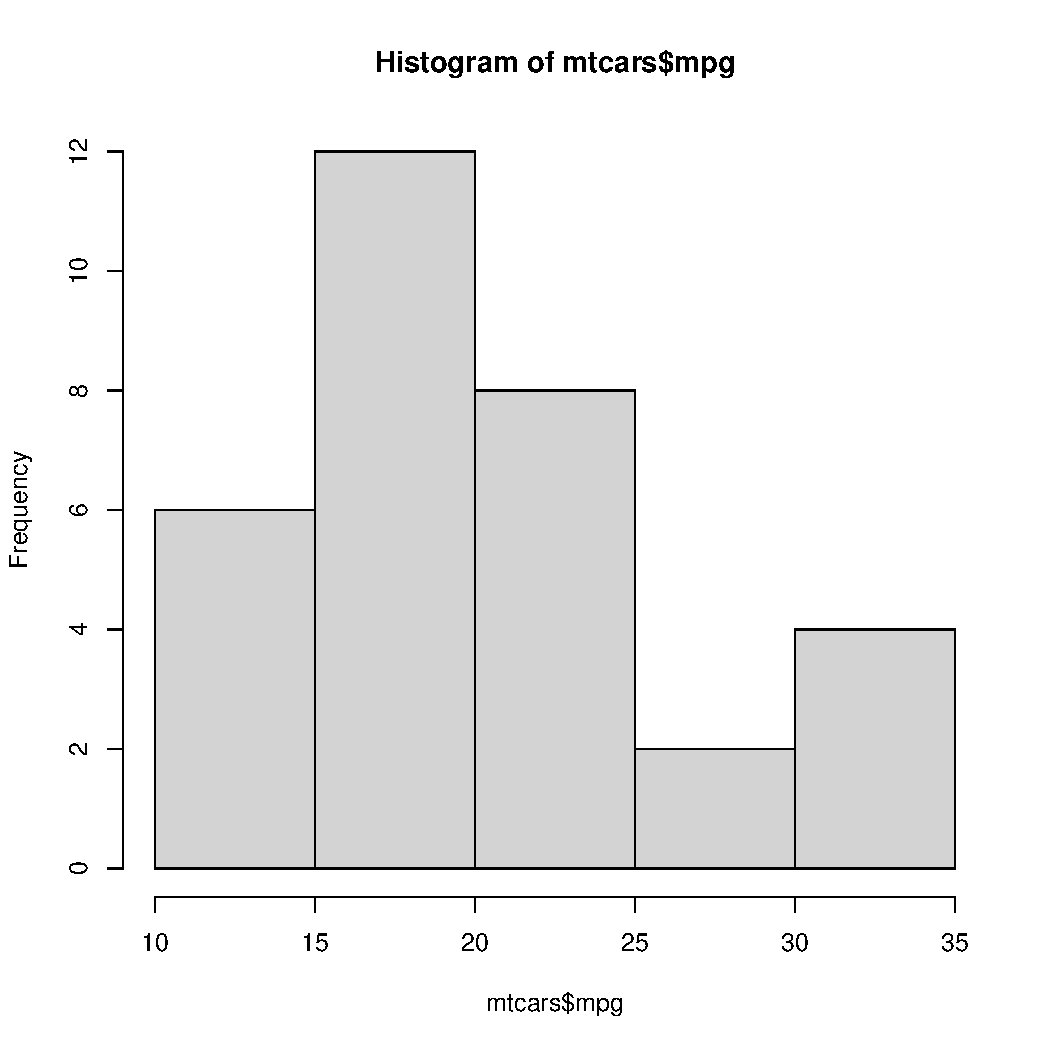
\includegraphics[width=\maxwidth]{figure/Q4-1} 
\begin{kframe}\begin{alltt}
\hlkwd{plot}\hlstd{(mtcars}\hlopt{$}\hlstd{wt, mtcars}\hlopt{$}\hlstd{mpg)}
\end{alltt}
\end{kframe}
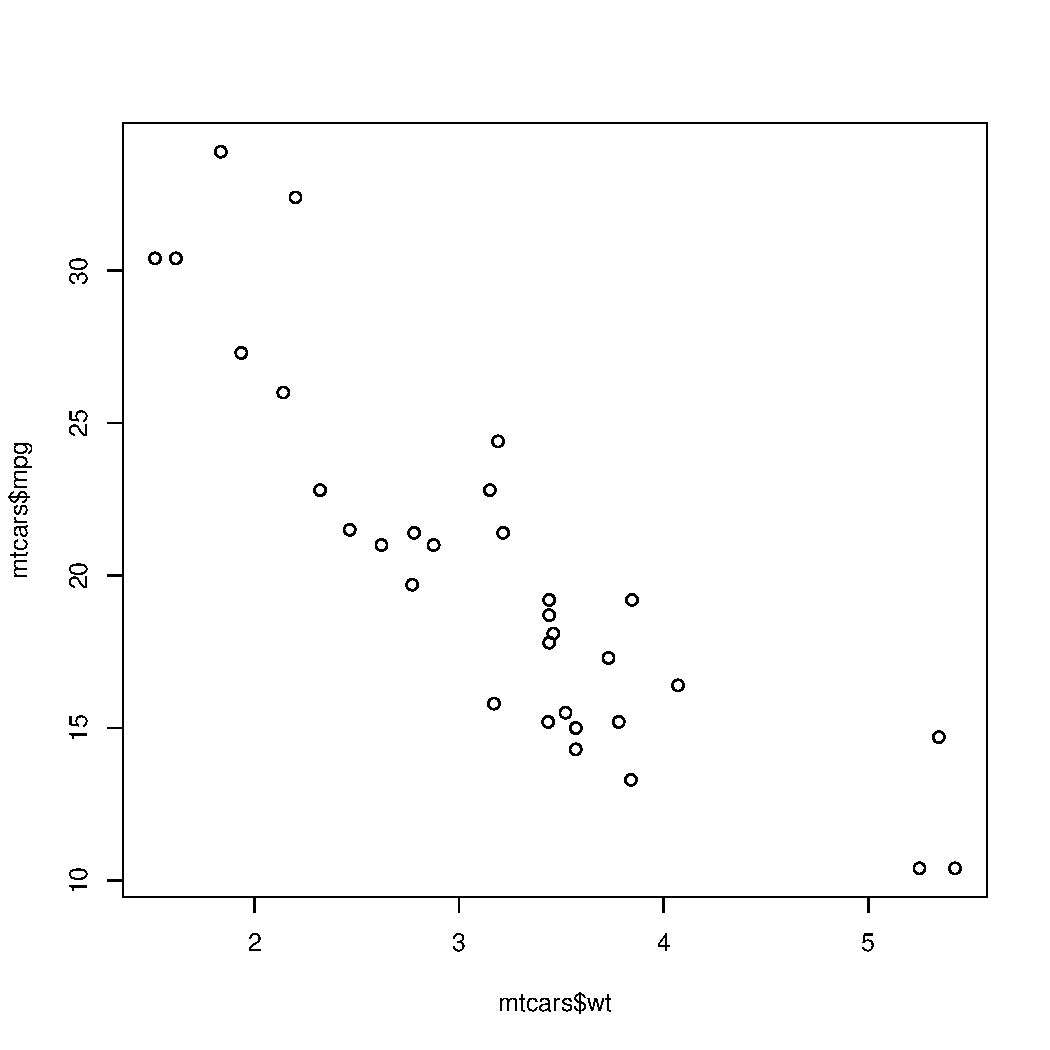
\includegraphics[width=\maxwidth]{figure/Q4-2} 
\end{knitrout}

5. **Advanced Analysis (Optional):**
   - Perform a linear regression analysis to study the relationship between mpg (as the dependent variable) and other variables like weight (`wt`), horsepower (`hp`), and number of cylinders (`cyl`). Use the `lm()` function for this.
   - Summarize your linear regression model using the `summary()` function and interpret the results.
\begin{knitrout}
\definecolor{shadecolor}{rgb}{0.969, 0.969, 0.969}\color{fgcolor}\begin{kframe}
\begin{alltt}
\hlkwd{library}\hlstd{(tidyverse)}
\hlcom{# Define the independent variables}
\hlstd{independent_vars} \hlkwb{<-} \hlkwd{c}\hlstd{(}\hlstr{"hp"}\hlstd{,} \hlstr{"cyl"}\hlstd{,} \hlstr{"drat"}\hlstd{,} \hlstr{"qsec"}\hlstd{,} \hlstr{"vs"}\hlstd{,} \hlstr{"carb"}\hlstd{)}
\hlcom{# Create a list of formulas}
\hlstd{formulas} \hlkwb{<-} \hlkwd{lapply}\hlstd{(}
  \hlstd{independent_vars,}
  \hlkwa{function}\hlstd{(}\hlkwc{var}\hlstd{)} \hlkwd{as.formula}\hlstd{(}\hlkwd{paste}\hlstd{(}\hlstr{"mpg ~"}\hlstd{, var))}
\hlstd{)}
\hlcom{# Use map() to apply lm() to each formula}
\hlstd{models} \hlkwb{<-} \hlkwd{map}\hlstd{(formulas,} \hlopt{~} \hlkwd{lm}\hlstd{(}\hlkwc{data} \hlstd{= mtcars,} \hlkwc{formula} \hlstd{= .))}
\hlcom{# Create a tibble with model summaries}
\hlstd{model_summaries} \hlkwb{<-} \hlkwd{tibble}\hlstd{(}\hlkwc{variable} \hlstd{= independent_vars,} \hlkwc{model} \hlstd{= models)} \hlopt
  \hlkwd{mutate}\hlstd{(}\hlkwc{summary} \hlstd{=} \hlkwd{map}\hlstd{(model, summary))}
\hlcom{# View the tibble}
\hlkwd{print}\hlstd{(model_summaries)}
\end{alltt}
\begin{verbatim}
## # A tibble: 6 x 3
##   variable model  summary   
##   <chr>    <list> <list>    
## 1 hp       <lm>   <smmry.lm>
## 2 cyl      <lm>   <smmry.lm>
## 3 drat     <lm>   <smmry.lm>
## 4 qsec     <lm>   <smmry.lm>
## 5 vs       <lm>   <smmry.lm>
## 6 carb     <lm>   <smmry.lm>
\end{verbatim}
\begin{alltt}
\hlkwd{walk}\hlstd{(model_summaries}\hlopt{$}\hlstd{summary, print)}
\end{alltt}
\begin{verbatim}
## 
## Call:
## lm(formula = ., data = mtcars)
## 
## Residuals:
##     Min      1Q  Median      3Q 
## -5.7121 -2.1122 -0.8854  1.5819 
##     Max 
##  8.2360 
## 
## Coefficients:
##             Estimate Std. Error
## (Intercept) 30.09886    1.63392
## hp          -0.06823    0.01012
##             t value Pr(>|t|)    
## (Intercept)  18.421  < 2e-16 ***
## hp           -6.742 1.79e-07 ***
## ---
## Signif. codes:  
##   0 '***' 0.001 '**' 0.01 '*'
##   0.05 '.' 0.1 ' ' 1
## 
## Residual standard error: 3.863 on 30 degrees of freedom
## Multiple R-squared:  0.6024,	Adjusted R-squared:  0.5892 
## F-statistic: 45.46 on 1 and 30 DF,  p-value: 1.788e-07
## 
## 
## Call:
## lm(formula = ., data = mtcars)
## 
## Residuals:
##     Min      1Q  Median      3Q 
## -4.9814 -2.1185  0.2217  1.0717 
##     Max 
##  7.5186 
## 
## Coefficients:
##             Estimate Std. Error
## (Intercept)  37.8846     2.0738
## cyl          -2.8758     0.3224
##             t value Pr(>|t|)    
## (Intercept)   18.27  < 2e-16 ***
## cyl           -8.92 6.11e-10 ***
## ---
## Signif. codes:  
##   0 '***' 0.001 '**' 0.01 '*'
##   0.05 '.' 0.1 ' ' 1
## 
## Residual standard error: 3.206 on 30 degrees of freedom
## Multiple R-squared:  0.7262,	Adjusted R-squared:  0.7171 
## F-statistic: 79.56 on 1 and 30 DF,  p-value: 6.113e-10
## 
## 
## Call:
## lm(formula = ., data = mtcars)
## 
## Residuals:
##     Min      1Q  Median      3Q 
## -9.0775 -2.6803 -0.2095  2.2976 
##     Max 
##  9.0225 
## 
## Coefficients:
##             Estimate Std. Error
## (Intercept)   -7.525      5.477
## drat           7.678      1.507
##             t value Pr(>|t|)    
## (Intercept)  -1.374     0.18    
## drat          5.096 1.78e-05 ***
## ---
## Signif. codes:  
##   0 '***' 0.001 '**' 0.01 '*'
##   0.05 '.' 0.1 ' ' 1
## 
## Residual standard error: 4.485 on 30 degrees of freedom
## Multiple R-squared:  0.464,	Adjusted R-squared:  0.4461 
## F-statistic: 25.97 on 1 and 30 DF,  p-value: 1.776e-05
## 
## 
## Call:
## lm(formula = ., data = mtcars)
## 
## Residuals:
##     Min      1Q  Median      3Q 
## -9.8760 -3.4539 -0.7203  2.2774 
##     Max 
## 11.6491 
## 
## Coefficients:
##             Estimate Std. Error
## (Intercept)  -5.1140    10.0295
## qsec          1.4121     0.5592
##             t value Pr(>|t|)  
## (Intercept)  -0.510   0.6139  
## qsec          2.525   0.0171 *
## ---
## Signif. codes:  
##   0 '***' 0.001 '**' 0.01 '*'
##   0.05 '.' 0.1 ' ' 1
## 
## Residual standard error: 5.564 on 30 degrees of freedom
## Multiple R-squared:  0.1753,	Adjusted R-squared:  0.1478 
## F-statistic: 6.377 on 1 and 30 DF,  p-value: 0.01708
## 
## 
## Call:
## lm(formula = ., data = mtcars)
## 
## Residuals:
##    Min     1Q Median     3Q    Max 
## -6.757 -3.082 -1.267  2.828  9.383 
## 
## Coefficients:
##             Estimate Std. Error
## (Intercept)   16.617      1.080
## vs             7.940      1.632
##             t value Pr(>|t|)    
## (Intercept)  15.390 8.85e-16 ***
## vs            4.864 3.42e-05 ***
## ---
## Signif. codes:  
##   0 '***' 0.001 '**' 0.01 '*'
##   0.05 '.' 0.1 ' ' 1
## 
## Residual standard error: 4.581 on 30 degrees of freedom
## Multiple R-squared:  0.4409,	Adjusted R-squared:  0.4223 
## F-statistic: 23.66 on 1 and 30 DF,  p-value: 3.416e-05
## 
## 
## Call:
## lm(formula = ., data = mtcars)
## 
## Residuals:
##    Min     1Q Median     3Q    Max 
## -7.250 -3.316 -1.433  3.384 10.083 
## 
## Coefficients:
##             Estimate Std. Error
## (Intercept)  25.8723     1.8368
## carb         -2.0557     0.5685
##             t value Pr(>|t|)    
## (Intercept)  14.085 9.22e-15 ***
## carb         -3.616  0.00108 ** 
## ---
## Signif. codes:  
##   0 '***' 0.001 '**' 0.01 '*'
##   0.05 '.' 0.1 ' ' 1
## 
## Residual standard error: 5.113 on 30 degrees of freedom
## Multiple R-squared:  0.3035,	Adjusted R-squared:  0.2803 
## F-statistic: 13.07 on 1 and 30 DF,  p-value: 0.001084
\end{verbatim}
\end{kframe}
\end{knitrout}

6. **Reflection:**
   - Write a brief summary of your findings. Which variables seem to affect mpg the most? Were there any surprises in your analysis?

**Deliverables:**
- R script with your code and comments explaining each step.
- A brief report summarizing your findings.

This exercise will help you practice data manipulation, conditional operations, basic plotting, and simple linear regression in R. It's a great way to get comfortable with some of the core functionalities of R using a well-known dataset. Remember, the best way to learn is by doing, so feel free to experiment with the data beyond the tasks listed here!

\end{document}
